%%%%%%%%%%%%%%%%%%%%%%%%%%%%%%%%%%%%%%%%%%%%%%%%%%%%%%%%%%%%%%%%%%%%%%%%%%%%%%%%%%%%%%%%%%%%%%%%%%%%%%%%%%%%%%%%%%%%%%%%%%%%%%%%%%%%%%%%%%%%%%%%%%%%%%%%%%%%%%%%%%%%%%%
%%%%%%%%%%%%%%%%%%%%%%%%%%%%%%%%%%%%%%%%%%%%%%%%%%%%%%%%%%%%%%%%%%%%%%%%%%%%%%%%%%%%%%%%%%%%%%%%%%%%%%%%%%%%%%%%%%%%%%%%%%%%%%%%%%%%%%%%%%%%%%%%%%%%%%%%%%%%%%%%%%%%%%%
%%%%%%%%%%%%%%%%%%%%%%%%%%%%%%%%%%%%%%%%%%%%%%%%%%%%%%%%%%%%%%%%%%%%%%%%%%%%%%%%%%%%%%%%%%%%%%%%%%%%%%%%%%%%%%%%%%%%%%%%%%%%%%%%%%%%%%%%%%%%%%%%%%%%%%%%%%%%%%%%%%%%%%%
%%%%%%%%%%%%%%%%%%%%%%%%%%%%%%%%%%%%%%%%%%%%%%%%%%%%%%%%%%%%%%%%%%%%%%%%%%%%%%%%%%%%%%%%%%%%%%%%%%%%%%%%%%%%%%%%%%%%%%%%%%%%%%%%%%%%%%%%%%%%%%%%%%%%%%%%%%%%%%%%%%%%%%%
\FloatBarrier
\chapter{Results}
\label{sec:Results}
After developing the methods of the background estimation for all different background sources and their corresponding systematic uncertainties (all explained in Section~\ref{ch:BackgroundEstimation}), 
the search is performed in four exclusive signal regions with 19.7\fbinv of data collected at a centre-of-mass energy of $\sqrt{s} = 8\tev$ at the CMS experiment.
The predicted numbers of events for the fake and the leptonic background in the four signal regions, as well as the number of observed events are listed in Table~\ref{tab:BackgroundPrediction}.
It can be seen, that fake tracks are by far the dominant background to this search.
The leptonic background contributes only in one signal region to the total background with a share of about 10\%.

Furthermore, the observations are compatible with the Standard Model background within 1$\sigma$ uncertainties in all four signal regions.
This is also visualised in Fig.~\ref{fig:FinalResult}, where a comparison of the total background prediction to the number of observed events is shown.
No excess above the SM prediction is observed in either of the four signal regions.
Thus, no evidence for physics beyond the Standard Model could be found.

Therefore, in the following section these results will be used to constrain the parameter space of supersymmetric models with almost mass-degenerate charginos and neutralinos.

\renewcommand{\arraystretch}{2.0}
\begin{table}[!h]
\centering
\caption{Number of predicted (fake, leptonic and total) and observed events for the four different signal regions.}
\label{tab:BackgroundPrediction}
\resizebox{\textwidth}{!}{
\begin{tabular}{c|c|ccc|ccc|ccc|c}
\multicolumn{5}{c}{} \\
\toprule
\multicolumn{2}{c|}{Signal region}     & \multicolumn{3}{c|}{Fake Bkg}  & \multicolumn{3}{c|}{ Leptonic Bkg}  &   \multicolumn{3}{c|}{ Total Bkg}   &   Data\\
\multicolumn{1}{c}{\pt [\gev]} & \ias  & \multicolumn{1}{c}{pred} & \multicolumn{1}{c}{stat} & sys & \multicolumn{1}{c}{pred} & \multicolumn{1}{c}{stat} & sys & \multicolumn{1}{c}{pred} & \multicolumn{1}{c}{stat} & sys   &        \\ 
\midrule
30-50                 & 0.05-0.30  & 19.11 &$^{+ 2.61} _{- 2.61}$ & $\pm$ 9.35  & 0.00 & $^{+ 2.58} _{- 0.00}$ & $\pm$ 0.00 &  19.11 &$^{+ 3.67} _{- 2.61}$ & $\pm$ 9.35 & 18\\
50-$\infty$           & 0.05-0.30  & 22.21 &$^{+ 3.60} _{- 3.60}$ & $\pm$ 8.78  & 2.17 & $^{+ 2.99} _{- 1.34}$ & $\pm$ 1.65 &  24.38 &$^{+ 4.68} _{- 3.84}$ & $\pm$ 8.93 & 34\\
30-50                 & 0.30-1.00  & 2.49  &$^{+ 0.85} _{- 0.85}$ & $\pm$ 1.98  & 0.00 & $^{+ 0.22} _{- 0.00}$ & $\pm$ 0.00 &  2.49  &$^{+ 0.87} _{- 0.85}$ & $\pm$ 1.98 & 0\\
50-$\infty$           & 0.30-1.00  & 2.52  &$^{+ 1.14} _{- 1.14}$ & $\pm$ 1.27  & 0.04 & $^{+ 0.30} _{- 0.03}$ & $\pm$ 0.03 &  2.57  &$^{+ 1.18} _{- 1.14}$ & $\pm$ 1.27 & 4 \\
\bottomrule
\multicolumn{5}{c}{}\\
\end{tabular}}
\end{table}

\begin{figure}[!b]
  \centering 
  \begin{tabular}{c}
    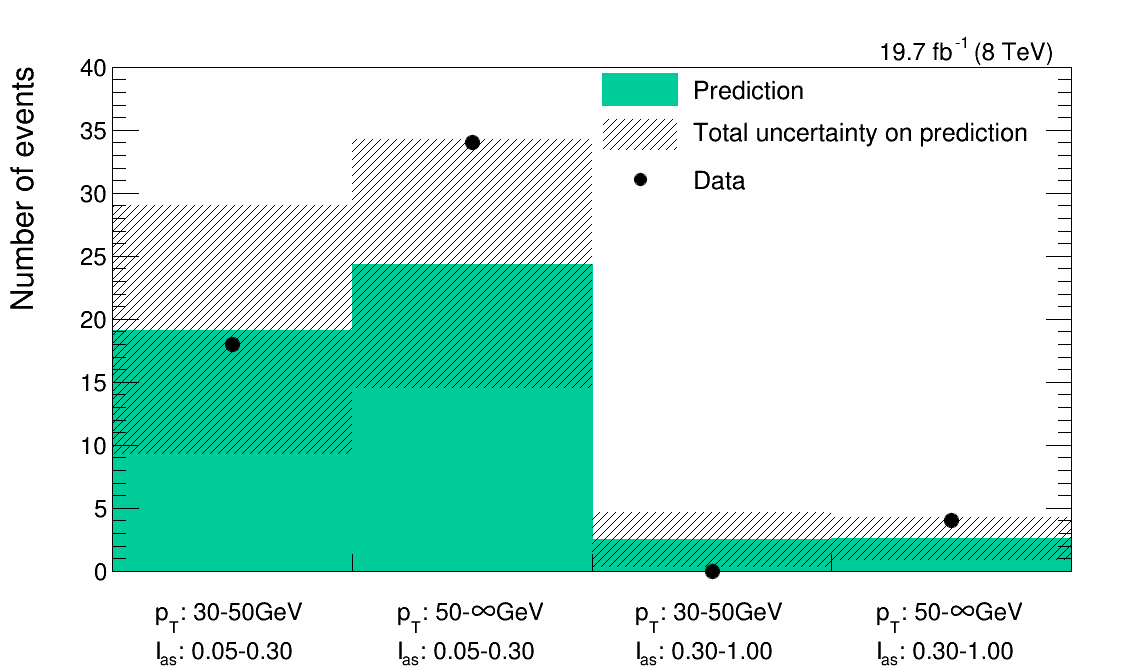
\includegraphics[width=0.98\textwidth]{figures/analysis/Results/FinalResultPlot.png} 
  \end{tabular}
  \caption{Number of predicted (green area) and observed (black dots) events for the four different signal regions. The hashed area represents the total uncertainty on the background prediction.}
  \label{fig:FinalResult}
\end{figure} 

%%%%%%%%%%%%%%%%%%%%%%%%%%%%%%%%%%%%%%%%%%%%%%%%%%%%%%%%%%%%%%%%%%%%%%%%%%%%%%%%%%%%%%%%%%%%%%%%%%%%%%%%%%%%%%%%%%%%%%%%%%%%%%%%%%%%%%%%%%%%%%%%%%%%%%%%%%%%%%%%%%%%%%%
%%%%%%%%%%%%%%%%%%%%%%%%%%%%%%%%%%%%%%%%%%%%%%%%%%%%%%%%%%%%%%%%%%%%%%%%%%%%%%%%%%%%%%%%%%%%%%%%%%%%%%%%%%%%%%%%%%%%%%%%%%%%%%%%%%%%%%%%%%%%%%%%%%%%%%%%%%%%%%%%%%%%%%%

